\chapter{Implementation}

The implementation should look at any issues you encountered as you tried to implement your design. During the work, you might have found that elements of your design were unnecessary or overly complex; perhaps third party libraries were available that simplified some of the functions that you intended to implement. If things were easier in some areas, then how did you adapt your project to take account of your findings?

It is more likely that things were more complex than you first thought. In particular, were there any problems or difficulties that you found during implementation that you had to address? Did such problems simply delay you or were they more significant? 

You can conclude this section by reviewing the end of the implementation stage against the planned requirements. 

\section{Initial work}
Development was carried out in weekly iterations starting from Monday 27th February 2017. To enable a smooth start to development, several tasks were completed before this, starting with setting up the development and testing environment.

To develop the charades game, both python and OpenCV needed to be set up. Installing python on windows is done by downloading the windows installer from the python.org website and running it - following the instructions on the installation wizard. 
...


\section{Iteration 1}
\textbf{Date}: 27/02/2017 \\
\textbf{Features}: 1, 3, 4 \\
\textbf{Overview}: The first iteration focused on putting in place the ground work for the hologram creation application. In addition to developing an understanding for the OpenCV library, tasks for this iteration also included obtaining and displaying a video feed from a web cam, as well as rotating the image obtained from the web cam.

\subsection{OpenCV API}
Due to the diversity of the OpenCV library with regards to its platform deployment and versioning, the documentation for the library is fragmented making examples difficult to find. Most documentation is basic and the online API covers all programming languages. It was for this reason, that much of the first iteration was spent deciphering the way the library should be used. The online documentation did provide a tutorial for the implemention of capturing the output from a web cam \cite{video_capture_tutorial}. This tutorial was used as a starting point for the system (Feature 1).

\subsection{Deep versus shallow copying}
Originally, the feature list contained an additional feature to be implemented during this iteration. The feature was to create 4 copies of the video feed to display them on each side of the pyramid. Original spike work suggested that this could involve creating a deep copy of the VideoCapture output. The reason a deep copy would be required is that each instance of the video feed would need to be rotated independently of the others. If the default operation for copying a video frame in Python is a shallow copy, then both variables will share a pointer to a single object \cite{deep_shallow_copying}. If this is the case, then rotating the video frame will rotate all the instances rather than just one. Through further investigation, it was discovered that each frame of the video was of type numpy array. Furthermore, the output window, where the video feeds were being displayed, was also a numpy array. This removes the problem of having to make a deep copy of the array as the numbers from the array can be directly added to the output array rather than copying the frames individually.

\newpage

\section{Iteration 2}
\textbf{Date}: 27/02/2017 \\
\textbf{Features}: 2, 5, 16 \\
\textbf{Overview}: The majority of work in this iteration involved investigation and implementation of a method for background subtraction in the charades game. This feature was estimated to take 3 or 4 days due to its complexity, as such minor features from the charades game were also added to this iteration.

\subsection{Background subtraction research}
To begin this iteration, research took place to determine the best possible method for background subtraction from the video frame. The "Comparative study of background subtraction algorithms" \cite{background_subtraction_comparison} provided an interesting summary and comparison of possible background subtraction routines. Given the need for real time execution of the background subtraction, it was decided to use the simple background subtraction technique. Simple background subtraction is performed by taking an image of the scene without the subject (foreground) present. For all frames that follow this, the background image is then subtracted from the frame which will leave only the foreground image.

\subsection{Image subtraction}
The simple background subtraction technique was implemented using the first frame captured by the web cam as the background image. Then when displayed, this image was subtracted from the real-time data from the web cam. Originally, this was implemented in full colour but due to the camera shake, auto focus and lighting adjustment made by the camera itself, the background image differed too much from the real-time foreground. To compensate for this, the background images was changed to be grey scale reducing the variance in colour from three channels to one. The grey scale background was then subtracted from a grey scale version of the web cam output and the resulting image was used as a mask. The mask could then be applied to the real-time video feed to only display the content that is outside of the mask. Using a mask improved the quality of the background subtraction, but not to the degree that was acceptable, as the mask that was generated was poor and contained holes due to the quality of the input video.

\subsection{Green screen}
The approach of using a green screen is commonly used in film and television production. This technique involves placing a green screen behind the object of interest, and then removing the green colour from the scene programmatically. The green colour is used for filming humans as it is a stark contrast to most skin tones. This implementation proved more effective in the quality of the output image produced. However, due to the video feed being captured in real-time, the function to remove the background needed fast execution to not reduce the frame rate of the display. The camera being used captured video at a frame rate of 60 frames per second (FPS). Applying the algorithm for removing the background reduced the frame rate to close to 10 FPS as each individual pixel had to be checked to find if the colour was part of the background or foreground. Despite attempts to optimise the algorithm, the best FPS achieved was 15.

The background subtraction algorithm implementation was left at this point to allow for other development to take place during this iteration. Planning allowed for work to continue on this during the next iteration providing no set backs were encountered. This was an acceptable decision as a fall-back plan of using a black curtain as the background in the scene could be used if required.

\subsection{Defining the phrases}
Instead of further development on the background subtraction implementation, ideas for possible phrases to be used in the charades game were gathered. This involved research into the types of books and films that are popular with a younger target audience. Most of the phrases were selected from the \textit{"100 best children's books"} list from BookTrust \cite{book_trust} and Sara Schmidt's \textit{"15 Best Kids Movies Of 2016"} publish on screenrant.com \cite{movies_2016}.

Feature 5 was pushed back to the next iteration due to the setbacks with the background subtraction algorithm.

\newpage

\section{Iteration 3}
\textbf{Date}: 06/03/2017 \\
\textbf{Features}: Spike work for Charades Game \\
\textbf{Roll-over features}: 5 \\
\textbf{Overview}: As well as completing the remaining work (Feature 5) from the previous iteration, this iteration covered the set up and spike work for android application development. Whilst in the end the Charades game was implemented as a web application, at this stage of the project, the design was for an android application. This decision will be discussed in more detail in \textbf{Iteration 4}. Finally, this iteration reopened the investigation into the optimisation of the background subtraction algorithm.

\subsection{Android setup}
Android Studio was the IDE chosen for Android development as it is one of the largest Android specific IDEs available. Furthermore, the online documentation for Android Studio provides multiple guides that help with the set up and implementation of a basic android app. After downloading and installing the IDE, the \textit{"Create an Android Project"} guide \cite{create_android_project} was followed to aid in the setup of a blank project. The tutorials that were available meant that spike work was completed quickly and yielded a basic prototype for the android application.

\subsection{Android status bar}


\begin{figure}[h!]
	\centering{
		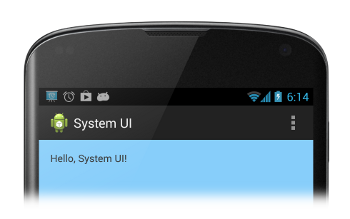
\includegraphics[scale=0.9]{Chapter3/status_bar_show.png}
		\caption{Shows a mock android application with the status bar open. The status bar is the black panel with the text "System UI" and the approve device information such as notification, signal, battery, ect. This image was taken from the "Hiding the Status Bar" tutorial created by the Android development team \cite{hide_status_bar}.}
		\label{fig:status_bar}
	}
\end{figure}


An additional task that was required alongside the creation of the welcome screen of the Android app was to remove the status bar from the Graphical User Interface (GUI). The status bar can be seen in Figure \ref{fig:status_bar} and the \textit{"Hiding the Status Bar"} tutorial \cite{hide_status_bar} from the Android developer site, gave an insight into how this could be removed from the app. When implementing the suggested changes from the tutorial, an error occurred routing from the call to the getActionBar() method that returns a pointer to the status bar. A stack overflow issue detailing this error \cite{sof_status_bar_err}, helped to diagnose the cause of the issue. The version of android being used was utilising the new
\begin{verbatim}
android.support.v7.app.ActionBarActivity
\end{verbatim}
which needed to be accessed as a support status bar rather than the older style regular status bar. This could be done using the function: 
\begin{verbatim}
getSupportActionBar()
\end{verbatim}

\subsection{UI testing}
To ensure that all elements of the Android application were subject to some form of automated testing, UI tests were developed for the Android app. These tests included checking page contents as well as page transitions to ensure that the expected content was visible and the buttons functioned correctly. As described in the Android developers guide \textit{"Testing Apps on Android"} \cite{testing_apps_on_android}, two types of test are commonly used for testing Android applications.

\begin{itemize}
	\item \textbf{Local unit tests}: Unit tests in this case are similar to any standard unit test for a normal code base. They test function input and output given various states. These tests are run on the local machine using the Java Virtual Machine (JVM) and have access to the Android specific API functions.
	
	\item \textbf{Instrumented tests}: By contrast, the Instrumented tests run on a hardware device or emulator. They are designed to test the app while it is running rather than testing individual functions, like a unit test. This allows for tests that exercise button transitions or page content to be run in an automated way.
\end{itemize}

For the UI testing, Instrumentation tests were developed and run on a mobile device attached to the development machine.

Whilst running tests for page content was straightforward, attempting to test page transitions proved more complex. A stack overflow issue was found that helped in to determine how this operation could be achieved \cite{sof_android_button_test}. The answer to the issue detailed using an ActivityMonitor class to listen for an Android Intent (the commands issued at the time of page transition) being executed.


\subsection{Background subtraction multi-threading}
Finally, this iteration revisited the background subtraction algorithm. Having already implemented the green screen algorithm, the algorithm or execution of the algorithm needed to be optimised to produce an acceptable frame rate. To do this, investigation in Python multi-threading took place. Each pixel in the input image needed to be checked and if it was above a certain value of green, changed to be black. This operation was performed on every pixel independently one after another. To improve the speed of execution, instead of checking the full array of the image in the main thread, the image was divided into 4 quadrants and each processed in a separate thread. Initially this was done in place in the array where each thread was given a start and end index to check. However, after implementing this solution, it was found to not have decreased the execution speed. This was the result of the array being locked while processing. To avoid multiple threads accessing the same numpy array and potential corrupting the data, the array is locked while one thread accesses it meaning that the next thread must wait for the first to finish. 

By creating new array objects that relate to each quadrant the lock problem was avoided, however only a slight decrease in execution time was found. More detailed investigation revealed that this was caused by the time taken to initialise new arrays with the data from each quadrant.

Again, as no solution was found for execution time issue, development of the background subtraction algorithm was halted. Instead it was decided to use a black background when filming. Whilst this solution offers less versatility in the location where actors can be filmed, it means that the frame rate of the hologram remains close to that of the camera feed. 

  
\newpage

\section{Iteration 4}
\textbf{Date}: 13/03/2017 \\
\textbf{Features}: 6, 7, 8 \\
\textbf{Overview}: Aberystwyth University Science Week was scheduled to begin on the 14th March 2017 and last a duration of three days. All the work required for the prototype (Feature 1-4) had been completed or alternative solutions found, as such it was possible to take the prototype to the event to test it with the target audience. In addition, this iteration concluded with a demonstration of the project so far on Friday 17th March. 

\subsection{Aberystwyth Science Week 2017}

\begin{figure}[h!]
	\centering{
		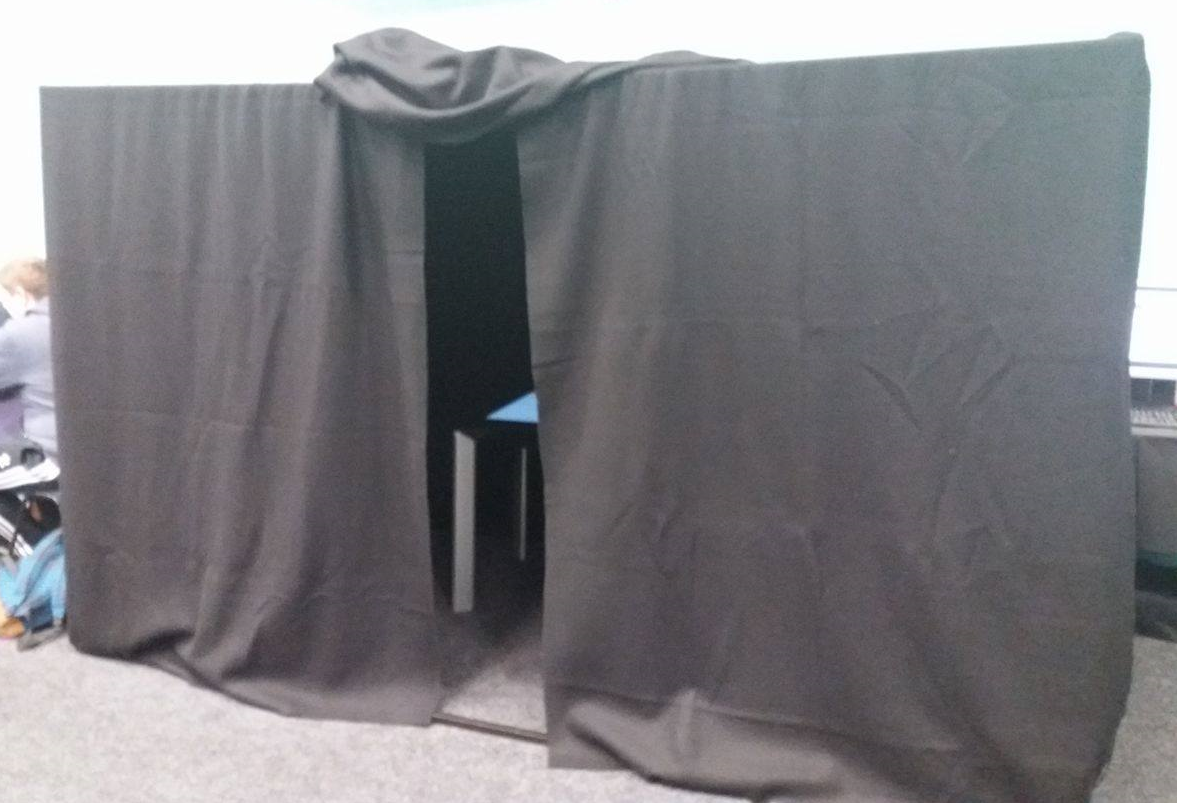
\includegraphics[scale=0.3]{Chapter3/viewing_area_science_week.png}
		\caption{Shows the viewing area for the real-time hologram creation system at the Aberystwyth University Science Week 2017. Inside, part of the touch screen table (being used as the display monitor for the system) is visible.}
		\label{fig:science_week_viewing_area}
	}
\end{figure}


The entities listed in the component diagram (the staging area, viewing area and image processing machine) were all constructed at the event venue. Figure \ref{fig:science_week_viewing_area} shows the viewing area (large black tent housing the monitor for the Pepper's Ghost Pyramid). To the right of the tent a camera attached to a computer was set up to record members of the audience. The camera was attached to the computer via a USB cable and the computer was attached to the external monitor in the tent via a HDMI cable.

Two main pieces of feedback could be inferred from using the prototype at the event. The first is that it proved a great success, with the clear majority of visiting students appearing greatly interested and engaged by the impactful display. The second was that students were not given much time at the event (most schools were present for an hour), meaning that the time that students were able to spend at each stall was limited. Originally, the Charades Game was designed to be played where actors and viewers would swap every time a correct answer was given, as would be the rules in a conventional game of charades. However, after discovering the limited time window for each activity at the science week, this concept was adjusted going forward to better suit the use case. To do this, two changes to the game rules were made:

\begin{itemize}
	 \item Actors act three phrases, and a points system was used, giving viewers points for correct guesses. At the end of each round, the viewer with the highest points would become the actor. This change enabled more time to be spent using the system, and less time for the member of the audience to be swapping roles.
	 
	 \item The subject of the phrase was changed to make more phrases single words and, rather than using conventional genres such as books and films, genres were changed to be activities and animals. These new genres meant a large amount of phrases were shorter and avoided long titles with simple words. A good example of where long titles would have been a problem is with the book "The Lion, the witch and the wardrobe". This phrase could take some time to act out fully due to the large number of words and it is also difficult to act simple words like "The".
\end{itemize} 

\subsection{Mid project demonstration and conclusions}
The mid project demonstration overall was a success and the demonstration of the software worked well. However, the question was raised as to why the charades system had been designed as an android application. The original reasoning for an android app was to promote the use of hand held devices for interaction with the system. Moreover, an Android app can potentially remove the reliance on the internet via the use of Bluetooth or locally connecting the devices together. This is an important factor to consider if, for example, an outreach event was being held in an area or building with poor reception. Furthermore, an android application removes problems that can occur with users attempting to manipulate the system via the URL which can be the case in some web apps.

Despite this, on re-evaluation of the project requirements and the final use case of the system, a web app was a better choice. The web app implementation removes many of the complications that could be faced with an android application which include:
\begin{itemize}
	\item Enabling devices to communicate with one another: Whilst there are many technologies for performing communications between android applications such as over the internet, via Bluetooth or through a peer-to-peer system, these technologies can be difficult to implement and test.
	\item Limiting the number of devices that are available: Whilst the event organisers would normally be able to get several tablets and mobile devices to use with the system. If users wished to join in on their own devices this would require that both the device they are using is on the android operating system, and the app is available on the Google Play Store.
\end{itemize}

A web app solves the above problems as it is already hosted on the internet which will allow for implicit communication between device accessing the system. Furthermore, the web app will be platform independent as the system code is executed server side and users interact with it through a web client.

Deciding to make this decision was difficult as due to the events of the week, little progress had been made on the android application. Starting again with a web application would mean further setbacks, but at the time the decision was made that it would lead to a better product.

\newpage

\section{Iteration 5}
\textbf{Date}: 20/03/2017 \\
\textbf{Features}: 9, 10 \\
\textbf{Roll-over features}: 5, 6, 7, 8 \\
\textbf{Overview}: This iterations first task was to adjust the features list schedule due to the decision to change to a web app from an Android app. Therefore, this iteration dealt with the roll over issues from the previous iterations, and Feature 9 and 10 (which were originally planned for this iteration) were redistributed among future iterations.

\subsection{Django}
As the hologram creation software already used the Python programming language it was logical to use a Python framework for implementation of the website. 

\subsection{}

Discussion points:
* Scrap App
* Investigation into Django
* Selenium testing
* Feature 5, 6, 7

\newpage

\section{Iteration 6}
\textbf{Date}: 27/03/2017 \\
\textbf{Features}: 9, 10, 11 \\
\textbf{Overview}:

Discussion points:
* Feature 8, 9, 10
* Session id

\newpage

\section{Iteration 7}
\textbf{Date}: 03/04/2017 \\
\textbf{Features}: 12, 13, 14 \\
\textbf{Overview}:

Discussion points:
* Feature 11, 12, 13
* polling

\newpage

\section{Iteration 8}
\textbf{Date}: 10/04/2017 \\
\textbf{Features}: 15, 17 \\
\textbf{Overview}:

Discussion points:
* Feature 14, 15, 17
* game conditions